\documentclass[11pt,letterpaper]{article}

\usepackage[margin=1in]{geometry}
\usepackage{hyperref}
\usepackage{booktabs}
\usepackage{longtable}
\usepackage{array}
\usepackage{xcolor}
\usepackage{listings}
\usepackage{tikz}
\usetikzlibrary{shapes.geometric, arrows.meta, positioning, fit, backgrounds, calc}
\usepackage{titlesec}
\usepackage{parskip}
\usepackage{microtype}
\usepackage{enumitem}

\hypersetup{
    colorlinks=true,
    linkcolor=blue!60!black,
    urlcolor=blue!60!black,
}

\lstset{
    basicstyle=\ttfamily\small,
    backgroundcolor=\color{gray!10},
    frame=single,
    breaklines=true,
    columns=fullflexible,
    keepspaces=true,
}

\titleformat{\section}{\large\bfseries}{}{0em}{}[\titlerule]
\titleformat{\subsection}{\normalsize\bfseries}{}{0em}{}

\title{\textbf{TermiNuke Battle Arena}\\[4pt]
       \large CSC209 Assignment 3 --- Systems Programming Mini-Project\\[2pt]
       \normalsize Project Documentation}
\date{}

\begin{document}
\maketitle
\thispagestyle{empty}
\tableofcontents
\newpage

%% ============================================================
\section{Project Overview}
%% ============================================================

TermiNuke is a multiplayer, turn-based, interactive battle arena played entirely inside the terminal. It falls under Category 2: Client-Server Application Using Sockets. Players connect to a server that hosts up to 64 independent game rooms. Each client first selects a room from a live room-list screen, then joins the lobby of that room. Once in the lobby, players select one of eight unique characters and battle against opponents using the character's available actions. The server records and broadcasts the status of the player and the battle process. When one player's HP reaches 0 or quits the game, the other player is declared the winner by the server.

\subsection*{What the application does}

The server tracks all game states, validates every player action, and resolves combat, which means that it handles basically all aspects of the game. Clients are basically just terminals that send player input and displays text through server broadcasts.

The game proceeds through phases that form a state machine (declared in \texttt{game.h}, lines~12--17):

\begin{enumerate}[leftmargin=2em]
    \item \textbf{Room Selection}: Immediately after TCP connection, the server sends \texttt{MSG\_ROOM\_LIST} to the new client. The client displays a table of all available rooms with their player count, status (Lobby / In Progress), and spectator count. The player types \texttt{join <room\_id>} to enter a specific room or \texttt{new} to be auto-assigned to an empty room.
    \item \textbf{Lobby}: Players connect to a room and select one of eight characters from a displayed roster indexed 0--7. Each character can only be picked once, which will be displayed as ``TAKEN''. The first player to join becomes the host.
    \item \textbf{Action Collection}: The host starts the game. Each round, every living player submits one action within a 30-second countdown timer. Some actions require a target to be an input during submission as well, which is indicated in the action description. The server accepts submissions at any time during this window and confirms each with a \texttt{MSG\_WAIT} acknowledgement.
    \item \textbf{Resolution}: When all actions are in or the timer expires (whichever comes first), the server executes moves in speed order. Speed is preset for each character and can be impacted with some actions. The moves to be executed are put in a queue of up to 16 narrative event strings, and they are released to every client at two-second intervals for dramatic effect.
    \item \textbf{Game Over}: The server announces the winner (or a tie if all remaining players are eliminated simultaneously) via \texttt{MSG\_GAME\_OVER}. The room then automatically resets to the lobby phase, and any spectators who were watching are promoted to lobby players for the next game.
\end{enumerate}

\subsection*{Spectator mode}

If a client selects a room that has a game already in progress, they join as a \emph{spectator} instead of a player. The server sends \texttt{MSG\_SPECTATE\_START} with a snapshot of the current game state. Spectators receive all subsequent game broadcasts (\texttt{MSG\_ROUND\_START}, \texttt{MSG\_TIMER\_TICK}, \texttt{MSG\_ROUND\_EVENT}, \texttt{MSG\_PLAYER\_ELIM}, \texttt{MSG\_GAME\_OVER}) exactly as players do. When the game ends, \texttt{promote\_spectators} (server.c, line~409) automatically transfers each spectator's file descriptor into an empty player slot and sends them \texttt{MSG\_JOIN\_ACK} and \texttt{MSG\_CHAR\_LIST}, seamlessly placing them in the lobby for the next round.

\subsection*{Input and output}

\textbf{Server}: No command line arguments are required. It listens on the port compiled in the \texttt{PORT} macro (default 4242). An optional \texttt{-r <num\_rooms>} flag sets the number of rooms (default 10, max 64). Game events are logged to \texttt{stdout}.

\textbf{Client}: The client is invoked as \texttt{./client <ip> <port>} and prompts the user for a player name before connecting. On connection, the client receives a room list and the user types \texttt{join <id>} or \texttt{new} to enter a room. Once in the lobby, they type \texttt{pick <id>} (0--7) to select a character. The host only needs to type \texttt{start} to begin. During each round, the user needs to type \texttt{<action\_id> [target\_id]} (e.g.\ \texttt{0}) to use their first move untargeted, or \texttt{2 3} to use their third move targeting player 3.

The client output has ANSI-coloured headers, a 20-character ASCII HP bar per player (rendered in \texttt{client.c}, \texttt{print\_hp\_bar}), and a typewriter-effect narrative display (15\,ms delay between characters, \texttt{typewriter\_print}) during resolution. Resolution refers to the time where the round ends and combat damage is calculated and messages are printed to the screen.

\subsection*{Key features}

There are eight playable characters (Albert Guo, Kaitlyn Zhu, Yibin Wang, Doug Ford, TTC, The Bitter TA, Jesus Christ, Karen Reid) and each carry four unique moves, for a total of 32 distinct abilities. A type-effectiveness matrix (five types: Student, Politician, Infrastructure, Teaching Staff, Divine) provides 1.5$\times$ damage multipliers. A status-effect system tracks over 30 independent per-player fields (poison, scrambled moves, shields, invulnerability, evasion, healing blocks, permanent buffs/debuffs, etc.) all defined in the \texttt{StatusEffects} struct in \texttt{game.h}.

Each character has actions with different effects. Actions can be categorized into 3 types: attack, defend, affect self, or opponent. (code: char\_def)
\begin{itemize}
    \item Attack-type: lower the opponent's HP
    \item Defend-type: reduce or eliminate the damage caused to self
    \item Effect-type: create positive (e.g., healing) or negative (e.g., increase next round's damage) effects to self or opponent.
\end{itemize}

\textbf{Type-effectiveness system} (\texttt{game.c} --- \texttt{get\_type\_effectiveness}):
Characters have a ``type''. Attacks from a certain type of character deal 1.5$\times$ damage to specific opposing types --- for example, a Teaching Staff-type attack deals 1.5$\times$ damage to a Student-type opponent. This feature is implemented via the \texttt{get\_type\_effectiveness} function in \texttt{game.c}, which encodes a fixed $5 \times 5$ advantage matrix and returns a multiplier of 1.5 when the attacker's type has an edge, or 1.0 otherwise.

\textbf{Multi-room server} (\texttt{server.c} --- \texttt{rooms[]}):
The server supports up to 64 simultaneous game rooms (10 by default, configurable with \texttt{-r}). Each room is an independent \texttt{GameState} and can hold up to 8 players and 16 spectators. Players are assigned to rooms explicitly via the room-selection screen, or auto-assigned to an empty room with the \texttt{new} command. All rooms run concurrently in the single-threaded event loop using \texttt{select}.

\textbf{Status effects} (\texttt{game.c} --- \texttt{game\_tick\_effects}):
Over 30 status effects are applied per-player each round by \texttt{game\_tick\_effects}. These include damage-over-time (poison), forced action skip (Drug Mixing), scrambled moves (Undefined Behaviour), forced miss (Dangling Pointer), evasion (Shuttle Buses / Notwithstanding), shields (Office Hours), healing blocks (Fare Inspector), and permanent stat changes (Gradient Descent, Buck-a-Beer, Man Page Reading), among others.

%% ============================================================
\section{Build Instructions}
%% ============================================================

The project builds with a single \texttt{make} invocation. All source files must be present in the same directory. No external libraries beyond the standard C library and \texttt{libm} are required.

\begin{lstlisting}
# Build both executables
make

# Optionally specify a different default port
make PORT=5000
\end{lstlisting}

This produces two executables: \texttt{server} and \texttt{client}.

\textbf{Running the server:}
\begin{lstlisting}
./server
# Server listens on 0.0.0.0:4242 with 10 rooms

# Optional: specify a different port or room count:
./server -p 5000
./server -p 5000 -r 4
\end{lstlisting}

\textbf{Running clients} (one terminal per player):
\begin{lstlisting}
./client 127.0.0.1 4242
\end{lstlisting}

\textbf{Minimum requirements:} 2 players must connect to the same room and select characters before the host can type \texttt{start}. Up to 8 players and 16 spectators can be in a room simultaneously. The server continues running indefinitely; each room resets to the lobby after a game ends.

\textbf{Compiler flags used} (see \texttt{Makefile}):
\begin{lstlisting}
gcc -Wall -Wextra -g -DPORT=4242 -o server server.c game.c -lm
gcc -Wall -Wextra -g -DPORT=4242 -o client client.c
\end{lstlisting}
\newpage
%% ============================================================
\section{Architecture Diagram}
%% ============================================================

The diagram below shows the server process, up to eight client processes per room, the TCP socket connections between them, and the categories of messages that flow in each direction. All communication is defined in \texttt{protocol.h}.

\begin{center}
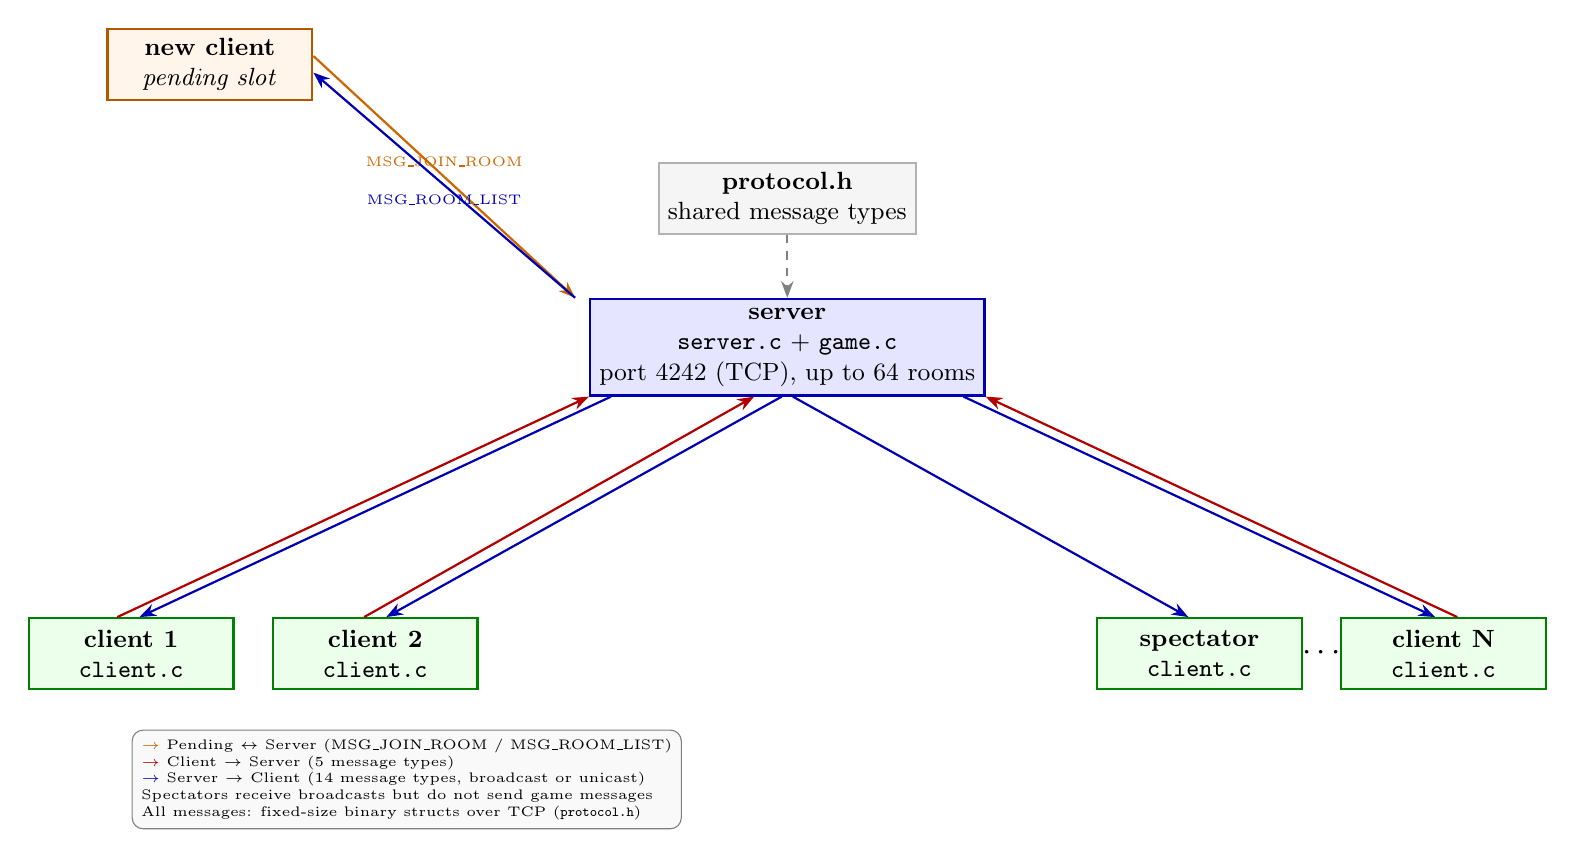
\begin{tikzpicture}[
    node distance=1.4cm and 2.2cm,
    every node/.style={font=\small},
    server/.style={rectangle, draw=blue!70!black, fill=blue!10, thick,
                   minimum width=4.2cm, minimum height=1.2cm, align=center},
    client/.style={rectangle, draw=green!50!black, fill=green!8, thick,
                   minimum width=2.6cm, minimum height=0.9cm, align=center},
    pending/.style={rectangle, draw=orange!70!black, fill=orange!8, thick,
                    minimum width=2.6cm, minimum height=0.9cm, align=center},
    file/.style={rectangle, draw=gray!60, fill=gray!8, thick,
                 minimum width=2.2cm, minimum height=0.8cm, align=center},
    arrow/.style={-{Stealth[length=6pt]}, thick},
    darrow/.style={{Stealth[length=6pt]}-{Stealth[length=6pt]}, thick},
]

%% --- Server box ---
\node[server] (srv) {\textbf{server}\\\texttt{server.c} + \texttt{game.c}\\port 4242 (TCP), up to 64 rooms};

%% --- Pending connection ---
\node[pending, above left=2.5cm and 3.5cm of srv] (pend)
    {\textbf{new client}\\\textit{pending slot}};

%% --- Lobby/game clients ---
\node[client, below left=2.8cm and 4.5cm of srv]  (c1) {\textbf{client 1}\\\texttt{client.c}};
\node[client, below left=2.8cm and 1.4cm of srv]  (c2) {\textbf{client 2}\\\texttt{client.c}};
\node[client, below right=2.8cm and 1.4cm of srv] (c3) {\textbf{spectator}\\\texttt{client.c}};
\node[client, below right=2.8cm and 4.5cm of srv] (c4) {\textbf{client N}\\\texttt{client.c}};

%% --- Dots ---
\node at ($(c3)!0.5!(c4)$) {\large$\cdots$};

%% --- Protocol header ---
\node[file, above=0.8cm of srv] (proto) {\textbf{protocol.h}\\shared message types};
\draw[arrow, dashed, gray] (proto) -- (srv);

%% --- Pending connection arrows ---
\draw[arrow, color=orange!80!black]
    ([yshift=3pt]pend.east) -- node[above, font=\tiny] {MSG\_JOIN\_ROOM} ([xshift=-5pt]srv.north west);
\draw[arrow, color=blue!70!black]
    ([xshift=-5pt]srv.north west) -- node[below, font=\tiny] {MSG\_ROOM\_LIST} ([yshift=-3pt]pend.east);

%% --- Arrows: client 1 ---
\draw[arrow, color=red!70!black]
    ([xshift=-5pt]c1.north) -- ([xshift=0pt]srv.south west);

\draw[arrow, color=blue!70!black]
    ([xshift=8pt]srv.south west) -- ([xshift=3pt]c1.north);

%% --- Arrows: client 2 ---
\draw[arrow, color=red!70!black]
    ([xshift=-4pt]c2.north) -- ([xshift=-12pt]srv.south);
\draw[arrow, color=blue!70!black]
    ([xshift=-2pt]srv.south) -- ([xshift=4pt]c2.north);

%% --- Arrows: spectator (receive only) ---
\draw[arrow, color=blue!70!black]
    ([xshift=2pt]srv.south) -- ([xshift=-4pt]c3.north);

%% --- Arrows: client N ---
\draw[arrow, color=red!70!black]
    ([xshift=5pt]c4.north) -- ([xshift=0pt]srv.south east);

\draw[arrow, color=blue!70!black]
    ([xshift=-8pt]srv.south east) -- ([xshift=-3pt]c4.north);

%% --- Legend ---
\node[draw=gray, fill=gray!5, rounded corners, font=\tiny, align=left,
      below=0.5cm of c1, xshift=3.5cm]
{
  \textcolor{orange!80!black}{$\rightarrow$} Pending $\leftrightarrow$ Server (MSG\_JOIN\_ROOM / MSG\_ROOM\_LIST)\\
  \textcolor{red!70!black}{$\rightarrow$} Client $\to$ Server (5 message types)\\
  \textcolor{blue!70!black}{$\rightarrow$} Server $\to$ Client (14 message types, broadcast or unicast)\\
  Spectators receive broadcasts but do not send game messages\\
  All messages: fixed-size binary structs over TCP (\texttt{protocol.h})
};

\end{tikzpicture}
\end{center}

The server's internal state machine (in \texttt{server.c} and \texttt{game.c}) is the sole source of truth. Clients maintain only the state required to render their UI and submit inputs. The \texttt{fd\_set} maintained in \texttt{main} (server.c, lines~1231--1256) tracks the listen socket, all pending connection sockets, all spectator sockets, and every active player socket across all rooms simultaneously.
\newpage

%% ============================================================
\section{Communication Protocol and Error Handling}
%% ============================================================

All messages are \textbf{fixed-width binary structs} defined in \texttt{protocol.h}. The first byte of every struct is always the \texttt{msg\_type} opcode. Because TCP is a stream protocol, both sides must know how many bytes to read; the opcode alone determines the struct type and thus the exact byte count expected. The server dispatches incoming messages from players in \texttt{process\_player\_buffer} (server.c, line~967) and from pending connections in \texttt{process\_pending\_buffer} (server.c, line~673); the client dispatches server messages in \texttt{process\_server\_buffer} (client.c). The \textbf{Error Handling} column below documents what occurs when a message is malformed, arrives in the wrong game state, or when the underlying \texttt{write(2)} or \texttt{read(2)} call fails.

\subsection*{Client $\to$ Server messages}

\begingroup
\small
\begin{longtable}{@{}p{1.8cm} p{1.2cm} p{2.4cm} p{4.2cm} p{4.8cm}@{}}
\toprule
\textbf{Message / Opcode} & \textbf{Size} & \textbf{Encoding} & \textbf{Semantics \& Invariants} & \textbf{Error Handling} \\
\midrule\endhead

\textbf{MSG\_JOIN\_ROOM}\\(0x05) &
36 bytes &
\texttt{uint8\_t msg\_type;}\newline
\texttt{uint8\_t room\_id;}\newline
\texttt{uint8\_t padding[2];}\newline
\texttt{char name[32];} &
Sent from a pending connection (before the client has joined any room). \texttt{room\_id} is 0--63, or \texttt{AUTO\_ROOM} (0xFF) to auto-assign to an empty lobby. \texttt{name} carries the player's chosen display name. If the target room is in \texttt{STATE\_LOBBY}, the client becomes a player; if a game is in progress, they become a spectator. &
\textbf{Server:} (1)~Invalid \texttt{room\_id} $\Rightarrow$ \texttt{MSG\_ERROR} + refreshed \texttt{MSG\_ROOM\_LIST} sent back (server.c:526--535). (2)~Lobby full $\Rightarrow$ \texttt{MSG\_ERROR} + \texttt{MSG\_ROOM\_LIST} (server.c:542--551). (3)~Too many spectators $\Rightarrow$ \texttt{MSG\_ERROR} + \texttt{MSG\_ROOM\_LIST} (server.c:614--624). (4)~\texttt{AUTO\_ROOM} with no empty room available $\Rightarrow$ \texttt{MSG\_ERROR} + \texttt{MSG\_ROOM\_LIST} (server.c:512--523). Non-printable bytes in \texttt{name} are sanitised to \texttt{'?'} (server.c:490--491); an empty name is replaced with ``Player''. \textbf{Client send:} \texttt{write\_all} failure $\Rightarrow$ \texttt{perror("write")} + \texttt{exit(1)} (client.c:514--516). \\[4pt]

\textbf{MSG\_JOIN}\\(0x01) &
33 bytes &
\texttt{uint8\_t msg\_type;}\newline
\texttt{char name[32];} &
Legacy opcode handled by \texttt{handle\_join} (server.c:794). Can be sent by already-slotted player fds. In the current client flow, players enter rooms via \texttt{MSG\_JOIN\_ROOM} instead; \texttt{MSG\_JOIN} is retained for compatibility but is not sent by the updated client. &
\textbf{Server:} (1)~Game already in progress $\Rightarrow$ \texttt{MSG\_ERROR} + close socket (server.c:798--804). (2)~Lobby full $\Rightarrow$ \texttt{MSG\_ERROR} + close socket (server.c:814--820). (3)~Non-printable bytes in \texttt{name} sanitised to \texttt{'?'} (server.c:810--811). \\[4pt]

\textbf{MSG\_ACTION}\\(0x02) &
4 bytes &
\texttt{uint8\_t msg\_type;}\newline
\texttt{uint8\_t action\_id;}\newline
\texttt{uint8\_t target\_id;}\newline
\texttt{uint8\_t padding;} &
Sent during \texttt{STATE\_ACTION\_COLLECTION} only. \texttt{action\_id} is 0--3. \texttt{target\_id} is forced to \texttt{NO\_TARGET} (0xFF) for untargeted moves. On success the server sends \texttt{MSG\_WAIT}. &
\textbf{Server:} (1)~Wrong game phase $\Rightarrow$ \texttt{MSG\_ERROR} ``Not currently accepting actions.''\ (server.c:881--885). (2)~Duplicate submission $\Rightarrow$ \texttt{MSG\_ERROR} ``You already submitted an action this round.''\ (server.c:886--890); original action preserved. (3)~Invalid \texttt{action\_id} or dead/out-of-range target $\Rightarrow$ \texttt{MSG\_ERROR} with specific string from \texttt{game\_validate\_action} (server.c:896--900); connection stays open so player can resubmit. \textbf{Client send:} \texttt{write\_all} failure $\Rightarrow$ \texttt{perror("write")} + \texttt{exit(1)} (client.c:580--583). Client also guards locally: a targeted move submitted without a target ID prints a usage hint without sending (client.c:567--572). \\[4pt]
\newpage

\textbf{MSG\_START\_GAME}\\(0x03) &
4 bytes &
\texttt{uint8\_t msg\_type;}\newline
\texttt{uint8\_t padding[3];} &
Sent by the host to begin the game. Only accepted during \texttt{STATE\_LOBBY} with $\geq$2 connected players, all having selected characters. &
\textbf{Server:} (1)~Non-host sender $\Rightarrow$ \texttt{MSG\_ERROR} ``Only the host can start.''\ (server.c:926--930); connection left open. (2)~Game already started $\Rightarrow$ \texttt{MSG\_ERROR} ``Game already started.''\ (server.c:931--935). (3)~Any connected player has no character $\Rightarrow$ \texttt{MSG\_ERROR} ``All players must select a character first.''\ (server.c:941--945). (4)~Fewer than 2 players $\Rightarrow$ \texttt{MSG\_ERROR} ``Need at least 2 players to start.''\ (server.c:950--954). In all four cases the game stays in \texttt{STATE\_LOBBY} and no state is mutated. \textbf{Client send:} \texttt{write\_all} failure $\Rightarrow$ \texttt{perror("write")} + \texttt{exit(1)} (client.c:467--470). \\[4pt]

\textbf{MSG\_CHAR\_SELECT}\\(0x04) &
4 bytes &
\texttt{uint8\_t msg\_type;}\newline
\texttt{uint8\_t char\_id;}\newline
\texttt{uint8\_t padding[2];} &
Sent during \texttt{STATE\_LOBBY} to claim character slot 0--7. On success, \texttt{MSG\_LOBBY\_UPDATE} and updated \texttt{MSG\_CHAR\_LIST} are broadcast to all players (server.c:864--870). &
\textbf{Server:} (1)~Not in lobby phase $\Rightarrow$ \texttt{MSG\_ERROR} ``Can't change character now.''\ (server.c:848--851); connection left open. (2)~\texttt{char\_id} out of range or character already taken $\Rightarrow$ \texttt{MSG\_ERROR} ``Character unavailable or invalid.''\ (server.c:854--857); player may retry with a different ID. \textbf{Client send:} \texttt{write\_all} failure $\Rightarrow$ \texttt{perror("write")} + \texttt{exit(1)} (client.c:452--455). \\
\bottomrule
\end{longtable}
\endgroup
\newpage

\subsection*{Server $\to$ Client messages}

\begingroup
\small
\begin{longtable}{@{}p{1.8cm} p{1.2cm} p{2.4cm} p{4.2cm} p{4.8cm}@{}}
\toprule
\textbf{Message / Opcode} & \textbf{Size} & \textbf{Encoding} & \textbf{Semantics \& Invariants} & \textbf{Error Handling} \\
\midrule\endhead

\textbf{MSG\_ROOM\_LIST}\\(0x1C) &
260 bytes &
\texttt{uint8\_t msg\_type;}\newline
\texttt{uint8\_t room\_count;}\newline
\texttt{uint8\_t padding[2];}\newline
\texttt{RoomInfo rooms[64];} &
Unicast to every new TCP connection immediately after \texttt{accept} (server.c:1350--1352). Also re-sent to a pending client when their \texttt{MSG\_JOIN\_ROOM} is rejected (invalid room, room full, etc.) so they can retry. Each \texttt{RoomInfo} (4 bytes) encodes room id, player count, phase, and spectator count. &
\textbf{Server write:} queued via \texttt{queue\_write\_pending} (server.c:1352); flushed the next time the pending fd appears in \texttt{wfds}. If \texttt{queue\_write\_pending} would overflow the 8\,KB pending write buffer, it returns \texttt{-1}; the accept loop does not check this return value, so in the extreme case the room list may be silently dropped. \textbf{Client receive:} triggers \texttt{on\_room\_list} (client.c:136), which sets \texttt{in\_room\_select = 1} and displays the room table; rooms with zero players and zero spectators are omitted from the display; always structurally valid. \\[4pt]

\textbf{MSG\_SPECTATE\_START}\\(0x1D) &
324 bytes &
\texttt{uint8\_t msg\_type;}\newline
\texttt{uint8\_t player\_count;}\newline
\texttt{uint8\_t round\_num;}\newline
\texttt{uint8\_t padding;}\newline
\texttt{PlayerInfo players[8];} &
Unicast to a client the moment they are placed in a spectator slot (server.c:665). Carries the current round number and a snapshot of all player HP, alive status, and character type so the spectator can immediately render the in-progress state. &
\textbf{Server write:} sent via \texttt{queue\_write\_spectator} inside \texttt{send\_spectate\_start} (server.c:394--403); flushed on the next \texttt{wfds} iteration. \textbf{Client receive:} triggers \texttt{on\_spectate\_start} (client.c:158), which sets \texttt{is\_spectator = 1}, \texttt{in\_room\_select = 0}, and renders the spectator view; always structurally valid. \\[4pt]

\textbf{MSG\_JOIN\_ACK}\\(0x19) &
4 bytes &
\texttt{uint8\_t msg\_type;}\newline
\texttt{uint8\_t your\_id;}\newline
\texttt{uint8\_t is\_host;}\newline
\texttt{uint8\_t room\_id;} &
Unicast to the connecting client immediately after \texttt{MSG\_JOIN\_ROOM} is processed (lobby path) or after a spectator is promoted to lobby player by \texttt{promote\_spectators}. \texttt{your\_id} is the player's slot (0--7); \texttt{is\_host} is 1 if this player is the game host; \texttt{room\_id} is the index of the room the client has joined, displayed in the lobby header. &
\textbf{Server write:} queued via \texttt{queue\_write} in \texttt{send\_join\_ack} (server.c:366--374); returns \texttt{-1} on failure. The caller checks the return value and calls \texttt{disconnect\_player} if the send fails, aborting the join sequence before any lobby broadcast occurs. \textbf{Client receive:} triggers \texttt{on\_join\_ack} (client.c:182), which sets \texttt{in\_room\_select = 0}, \texttt{is\_spectator = 0}, and stores \texttt{my\_room\_id} so the lobby header can display the current room number; always structurally valid. \\[4pt]

\textbf{MSG\_CHAR\_LIST}\\(0x1A) &
$\approx$13\,KB &
\texttt{uint8\_t msg\_type;}\newline
\texttt{uint8\_t char\_count;}\newline
\texttt{uint8\_t padding[2];}\newline
\texttt{CharEntry chars[8];} &
Unicast on join and broadcast after every character selection. Each \texttt{CharEntry} (protocol.h) contains stats and all four \texttt{ActionDef} entries. The \texttt{taken} field marks already-claimed characters. &
\textbf{Server write:} sent via \texttt{queue\_write} in \texttt{send\_char\_list} (server.c:255--263); returns \texttt{-1} on failure. All callers (\texttt{handle\_join\_room}, \texttt{handle\_char\_select}, \texttt{promote\_spectators}) check the return value and call \texttt{disconnect\_player} on failure. \textbf{Client receive:} always structurally valid. \\[4pt]

\textbf{MSG\_LOBBY\_UPDATE}\\(0x10) &
$\approx$324 bytes &
\texttt{uint8\_t msg\_type;}\newline
\texttt{uint8\_t player\_count;}\newline
\texttt{uint8\_t host\_id;}\newline
\texttt{uint8\_t padding;}\newline
\texttt{PlayerInfo players[8];} &
Broadcast to all clients whenever the lobby changes (player joins, leaves, or picks a character). Each \texttt{PlayerInfo} (40 bytes) encodes player id, hp, alive flag, char type, speed, max hp, char id, and name. &
\textbf{Server write:} sent via \texttt{broadcast} (server.c:199); \texttt{queue\_write} failure for any slot $\Rightarrow$ \texttt{disconnect\_player} called immediately for that slot; remaining players continue to receive the update uninterrupted. \textbf{Client receive:} always structurally valid. \\[4pt]
\newpage
\textbf{MSG\_GAME\_START}\\(0x11) &
$\approx$1.4\,KB &
\texttt{uint8\_t msg\_type;}\newline
\texttt{uint8\_t your\_id;}\newline
\texttt{uint8\_t player\_count;}\newline
\texttt{uint8\_t action\_count;}\newline
\texttt{PlayerInfo players[8];}\newline
\texttt{ActionDef actions[4];} &
Unicast to each player (server.c:265--285). \texttt{actions} carries the four moves for \emph{that player's} chosen character so the client can display them without hardcoding game data. &
\textbf{Server write:} sent per-player via \texttt{queue\_write} (server.c:282); the return value is checked for each player, and \texttt{disconnect\_player} is called immediately on failure. \textbf{Client receive:} always structurally valid; stores \texttt{my\_id} and the action list for the remainder of the session. \\[4pt]

\textbf{MSG\_ROUND\_START}\\(0x12) &
$\approx$324 bytes &
\texttt{uint8\_t msg\_type;}\newline
\texttt{uint8\_t round\_num;}\newline
\texttt{uint8\_t timer\_secs;}\newline
\texttt{uint8\_t player\_count;}\newline
\texttt{PlayerInfo players[8];} &
Broadcast to all players \emph{and spectators} at the start of every action-collection phase via \texttt{broadcast\_all} (server.c:296). Contains a fresh snapshot of all player HP, speed, and alive status. &
\textbf{Server write:} sent via \texttt{broadcast\_all}; \texttt{queue\_write} failure $\Rightarrow$ \texttt{disconnect\_player} or \texttt{disconnect\_spectator}. \textbf{Client receive:} resets per-round state flags (\texttt{waiting\_for\_result}, \texttt{in\_resolution}) and sets \texttt{need\_prompt = 1} for players (spectators receive the update but suppress the action prompt); always structurally valid. \\[4pt]

\textbf{MSG\_TIMER\_TICK}\\(0x13) &
4 bytes &
\texttt{uint8\_t msg\_type;}\newline
\texttt{uint8\_t seconds\_left;}\newline
\texttt{uint8\_t padding[2];} &
Broadcast to players and spectators once per second during action collection (server.c:1394--1396). When \texttt{seconds\_left} reaches 0 the server proceeds to resolution regardless of missing submissions. &
\textbf{Server write:} sent via \texttt{broadcast\_all} (server.c:306); \texttt{queue\_write} failure $\Rightarrow$ \texttt{disconnect\_player} or \texttt{disconnect\_spectator}. \textbf{Client receive:} always structurally valid; updates the countdown display or a ``waiting'' status line depending on \texttt{waiting\_for\_result}. \\[4pt]

\textbf{MSG\_ROUND\_EVENT}\\(0x14) &
260 bytes &
\texttt{uint8\_t msg\_type;}\newline
\texttt{uint8\_t padding[3];}\newline
\texttt{char text[256];} &
Broadcast to players and spectators during resolution, one event every two seconds (\texttt{RESOLVE\_DELAY\_US}\,=\,2\,000\,000\,$\mu$s, server.c:25). Each event is a null-terminated narrative string describing one combat action. &
\textbf{Server write:} sent via \texttt{broadcast\_all} (server.c:315); \texttt{queue\_write} failure $\Rightarrow$ \texttt{disconnect\_player} or \texttt{disconnect\_spectator}. \textbf{Client receive:} always structurally valid; sets \texttt{in\_resolution = 1}, which suppresses the action prompt until the next \texttt{MSG\_ROUND\_START} is received. \\[4pt]
\newpage

\textbf{MSG\_STATUS\_UPDATE}\\(0x1B) &
516 bytes &
\texttt{uint8\_t msg\_type;}\newline
\texttt{uint8\_t padding[3];}\newline
\texttt{char text[512];} &
Unicast to each living player at the start of every round (server.c:1074--1082). Contains a human-readable summary of active status effects built by \texttt{game\_build\_status\_text} (game.c). &
\textbf{Server write:} sent via \texttt{queue\_write} only to players with \texttt{alive \&\& fd != -1} (server.c:1076--1081); the return value is checked and \texttt{disconnect\_player} is called on failure. \textbf{Client receive:} always structurally valid. \\[4pt]

\textbf{MSG\_PLAYER\_ELIM}\\(0x15) &
36 bytes &
\texttt{uint8\_t msg\_type;}\newline
\texttt{uint8\_t player\_id;}\newline
\texttt{uint8\_t padding[2];}\newline
\texttt{char name[32];} &
Broadcast to players and spectators when a player's HP reaches zero or they disconnect mid-game. Clients display a ``player eliminated'' notification. &
\textbf{Server write:} sent via \texttt{broadcast\_all} (server.c:334); \texttt{queue\_write} failure $\Rightarrow$ \texttt{disconnect\_player} or \texttt{disconnect\_spectator}. \textbf{Client receive:} always structurally valid. \\[4pt]

\textbf{MSG\_GAME\_OVER}\\(0x16) &
36 bytes &
\texttt{uint8\_t msg\_type;}\newline
\texttt{uint8\_t is\_tie;}\newline
\texttt{uint8\_t winner\_id;}\newline
\texttt{uint8\_t padding;}\newline
\texttt{char winner\_name[32];} &
Broadcast to players and spectators when one (or zero) players remain. \texttt{is\_tie} is 1 if multiple players eliminated simultaneously; \texttt{winner\_id} is 0xFF on a tie. After broadcasting, the server resets the room to \texttt{STATE\_LOBBY} and calls \texttt{promote\_spectators}. &
\textbf{Server write:} sent via \texttt{broadcast\_all} (server.c:346); \texttt{queue\_write} failure $\Rightarrow$ \texttt{disconnect\_player} or \texttt{disconnect\_spectator}. After this message the server resets to lobby and spectators are promoted. \textbf{Client receive:} sets \texttt{game\_over = 1} and displays the result; always structurally valid. \\[4pt]
\newpage

\textbf{MSG\_WAIT}\\(0x18) &
4 bytes &
\texttt{uint8\_t msg\_type;}\newline
\texttt{uint8\_t padding[3];} &
Unicast acknowledgement sent to a player after their \texttt{MSG\_ACTION} is accepted (server.c:913). Signals the client to stop prompting for input and wait for resolution. &
\textbf{Server write:} sent via \texttt{queue\_write} in \texttt{send\_wait} (server.c:358--364); returns \texttt{-1} on failure. The caller in \texttt{handle\_action} checks the return value and calls \texttt{disconnect\_player} on failure. The player's \texttt{pending\_action\_id} is recorded \emph{before} the send (server.c:910--911), so the action is preserved even if delivery fails. \textbf{Client receive:} sets \texttt{waiting\_for\_result = 1} and suppresses further input prompts; always structurally valid. \\[4pt]

\textbf{MSG\_ERROR}\\(0x17) &
68 bytes &
\texttt{uint8\_t msg\_type;}\newline
\texttt{uint8\_t padding[3];}\newline
\texttt{char message[64];} &
Unicast error string for invalid actions, bad character selections, unauthorised start requests, rejected room joins, and connection-refused conditions. Fatal errors are followed immediately by socket close or a refreshed room list. &
\textbf{Server write:} sent via \texttt{queue\_write} in \texttt{send\_error} (server.c:349--356); returns \texttt{-1} on failure. For non-fatal errors sent to registered players (e.g.\ invalid actions, bad character selections), the caller checks the return value and calls \texttt{disconnect\_player} on failure. For rejected room-join attempts from pending connections, the server re-sends \texttt{MSG\_ROOM\_LIST} immediately after the error so the client can retry. \textbf{Client receive:} prints the message in red (\texttt{on\_error}, client.c); connection stays open for non-fatal errors so the player may retry. \\
\bottomrule
\end{longtable}
\endgroup

\subsection*{Message framing}

Because TCP is a byte stream, partial writes are possible. Both sides use a \texttt{write\_all} helper (server.c, line~69; client.c, line~47) that loops on \texttt{write(2)} until all bytes are sent or an error occurs. On the receive side the server maintains a 256-byte per-player read buffer (\texttt{Player.rbuf}, game.h) and a per-pending-connection read buffer (\texttt{PendingConn.rbuf}) that accumulate partial reads; \texttt{process\_player\_buffer} (server.c, line~967) and \texttt{process\_pending\_buffer} (server.c, line~673) each check whether a full message is present before dispatching, and call \texttt{memmove} to compact the buffer afterwards. When a pending connection is promoted to a player slot, only the bytes \emph{following} the already-processed \texttt{MSG\_JOIN\_ROOM} are transferred into the player's rbuf, preventing stale opcode bytes from being re-dispatched (server.c:571--577). The client uses a single 8\,KB \texttt{rbuf} (client.c, line~28) for the same purpose.

\subsection*{Cross-cutting error handling}

The following concerns affect the protocol as a whole rather than any individual message type.

\textbf{1. Client disconnection mid-game.} Every \texttt{read} on a player socket is checked for $n \leq 0$ (server.c, line~1441--1451). Zero means a clean peer close; negative means an I/O error (with an \texttt{EAGAIN}/\texttt{EWOULDBLOCK} exception for non-blocking sockets, which simply causes the read to be skipped). In both fatal cases \texttt{disconnect\_player} is called (server.c, line~1445), which closes the socket, sets \texttt{fd = -1} to remove it from the \texttt{fd\_set} on the next iteration, and frees the character slot. If the game is in progress, \texttt{game\_remove\_player} marks the player as eliminated and \texttt{MSG\_PLAYER\_ELIM} is broadcast to remaining players. \texttt{game\_check\_end} handles the edge case where a disconnect reduces survivors to one.

\textbf{2. Unknown or malformed opcode.} In \texttt{process\_player\_buffer} (server.c, line~980--984), the \texttt{default} branch logs the unknown opcode and immediately calls \texttt{disconnect\_player}, preventing the server from interpreting arbitrary bytes as valid messages and corrupting game state. Similarly, in \texttt{process\_pending\_buffer} (server.c, line~682--688), an unknown opcode causes \texttt{disconnect\_pending} to be called. Symmetrically, in \texttt{process\_server\_buffer} (client.c), an unknown server opcode causes a return of \texttt{-1}, which breaks the client event loop and closes the socket.

\textbf{3. Write failures (broken pipe).} All outbound data is routed through \texttt{queue\_write} (server.c, line~39) and flushed by \texttt{flush\_wbuf} (server.c, line~51). \texttt{flush\_wbuf} returns \texttt{-1} on any fatal \texttt{write(2)} failure including \texttt{EPIPE}. Equivalent helpers exist for pending connections (\texttt{queue\_write\_pending}, \texttt{flush\_wbuf\_pending}) and spectators (\texttt{queue\_write\_spectator}, \texttt{flush\_wbuf\_spectator}). Broadcast helpers that use \texttt{broadcast\_all} check the return value of \texttt{queue\_write} per player and call \texttt{disconnect\_player} or \texttt{disconnect\_spectator} on failure. If \texttt{queue\_write} detects that the 8\,KB buffer would overflow, it also returns \texttt{-1}, disconnecting the client. This design means a slow or unresponsive client can never stall the server.

\textbf{4. Socket setup failures.} Every system call in the server startup sequence---\texttt{socket}, \texttt{setsockopt}, \texttt{bind}, and \texttt{listen}---checks its return value and calls \texttt{perror} followed by \texttt{exit(1)} on failure (server.c, lines~1188--1205). The client similarly checks \texttt{socket}, \texttt{inet\_pton}, and \texttt{connect} (client.c, lines~612--627).

\textbf{5. \texttt{select} interrupted by signal (EINTR).} Both the server (server.c, line~1301) and the client (client.c, line~641) check \texttt{errno == EINTR} after a negative \texttt{select} return and restart the loop with a \texttt{continue}. Any other negative return is treated as fatal and reported with \texttt{perror}:
\begin{lstlisting}
if (ready < 0) {
    if (errno == EINTR) continue;
    perror("select"); exit(1);
}
\end{lstlisting}

\textbf{6. Client stdin EOF.} In both the lobby handler (client.c, line~438--441), the room-select handler (client.c, line~500--503), and the in-game handler (client.c, line~540--543), a \texttt{NULL} return from \texttt{fgets} closes the socket and calls \texttt{exit(0)}. Closing the socket triggers \texttt{read} returning 0 on the server, which invokes \texttt{disconnect\_player} or \texttt{disconnect\_pending} and handles the departure identically to any other disconnection.

\textbf{7. Player eliminated by status-effect tick before action collection.} \texttt{begin\_round} (server.c, line~1015) calls \texttt{game\_tick\_effects} and then immediately calls \texttt{game\_check\_end} before transitioning to \texttt{STATE\_ACTION\_COLLECTION}. If the check returns non-zero (one or zero survivors), the server broadcasts \texttt{MSG\_PLAYER\_ELIM} for each newly dead player, resets to \texttt{STATE\_LOBBY}, promotes spectators, and sends \texttt{MSG\_GAME\_OVER} without opening the action-collection window, ensuring the game always terminates cleanly even when damage-over-time effects deliver the killing blow between rounds.

\textbf{8. SIGPIPE suppression.} Writing to a TCP socket whose peer has closed produces a \texttt{SIGPIPE} signal, which by default terminates the process. The server installs \texttt{signal(SIGPIPE, SIG\_IGN)} at the top of \texttt{main} (server.c, line~1166) so that \texttt{write(2)} returns \texttt{-1} with \texttt{errno == EPIPE} instead. The existing \texttt{flush\_wbuf} and \texttt{queue\_write} error paths already check for negative return values and route through \texttt{disconnect\_player}, so once \texttt{SIGPIPE} is suppressed the broken-pipe case is handled identically to any other write failure---no special-case code is needed.
\newpage

%% ============================================================
\section{Concurrency Model}
%% ============================================================

The server is \textbf{single-process, single-threaded}. It uses a single \texttt{select(2)} call to monitor all file descriptors simultaneously, never blocking on any one client. No \texttt{fork} or \texttt{pthread} calls are made; concurrency is achieved entirely through I/O multiplexing.

\subsection*{The \texttt{fd\_set} contents}

At the top of the main event loop (server.c, lines~1224--1256) the server rebuilds \texttt{rfds} and \texttt{wfds} on every iteration:

\begin{itemize}[leftmargin=2em]
    \item \textbf{The listen socket} (\texttt{listen\_fd}) --- added to \texttt{rfds} to monitor for new incoming TCP connections.
    \item \textbf{All pending connection sockets} (up to 64) --- added to \texttt{rfds} for incoming \texttt{MSG\_JOIN\_ROOM} data, and to \texttt{wfds} if their write buffer is non-empty (\texttt{wbuf\_len > 0}) so that \texttt{MSG\_ROOM\_LIST} or error messages can be flushed asynchronously (server.c:1249--1256).
    \item \textbf{All active player sockets} (up to 8 per room, across all rooms) --- added to \texttt{rfds} for incoming data. Any player socket with a non-empty write buffer is also added to \texttt{wfds} so the server can flush pending outbound data as soon as the kernel is ready to accept it (server.c:1231--1239).
    \item \textbf{All spectator sockets} (up to 16 per room, across all rooms) --- added to \texttt{rfds} for disconnection detection, and to \texttt{wfds} if their write buffer is non-empty so that game-event messages forwarded to spectators are flushed asynchronously (server.c:1240--1248).
\end{itemize}

\subsection*{Timeout logic}

\texttt{select} is called with a baseline \texttt{struct timeval} of 100\,ms (server.c, lines~1260--1263). Before calling \texttt{select}, the server iterates over all rooms and refines the timeout downward (server.c, lines~1265--1297):

\begin{itemize}[leftmargin=2em]
    \item \textbf{\texttt{STATE\_ACTION\_COLLECTION}}: room requests a 1-second timeout. The server decrements \texttt{timer\_secs\_left} each second, broadcasts \texttt{MSG\_TIMER\_TICK}, and if the timer reaches zero calls \texttt{start\_resolution} immediately.
    \item \textbf{\texttt{STATE\_RESOLVING}}: room requests a timeout equal to the time remaining until the next 2-second event slot, computed using \texttt{gettimeofday}. When the timeout fires the server sends the next queued narrative event (\texttt{MSG\_ROUND\_EVENT}) and updates \texttt{resolve\_last\_send}.
    \item \textbf{\texttt{STATE\_LOBBY} / \texttt{STATE\_GAME\_OVER}}: no reduction; the 100\,ms baseline is used (effectively polling, allowing new connections and messages to be processed promptly even when all rooms are idle).
\end{itemize}

The minimum timeout across all rooms wins, so a single \texttt{select} call services every active timer simultaneously.

\subsection*{Non-blocking I/O and the write buffer}

Every accepted socket (players, pending connections, spectators) is set to \texttt{O\_NONBLOCK} via \texttt{set\_nonblocking} (server.c, line~31) immediately after \texttt{accept}. This guarantees that neither \texttt{read} nor \texttt{write} can block the server on a single slow client.

On the \textbf{read side}, every \texttt{read} is gated behind \texttt{FD\_ISSET}, so the server never attempts a read on a socket that has no data. For non-blocking player sockets, \texttt{EAGAIN}/\texttt{EWOULDBLOCK} is explicitly handled as a non-fatal condition (server.c:1444), which is important when a pending connection is promoted to a player slot within the same \texttt{select} iteration and the new player fd appears ready but has no new data.

On the \textbf{write side}, the server never calls \texttt{write(2)} directly on a client socket during message dispatch. Instead, all send helpers call \texttt{queue\_write} (or \texttt{queue\_write\_pending} / \texttt{queue\_write\_spectator}), which appends the message to the client's 8\,KB write buffer. After \texttt{select} returns, any socket that appears in \texttt{wfds} is flushed by the appropriate \texttt{flush\_wbuf} variant, which handles \texttt{EAGAIN}/\texttt{EWOULDBLOCK} by returning immediately---the remaining data stays in the buffer and is retried on the next \texttt{select} iteration. This design means a slow or unresponsive client can never stall the server; data accumulates in the per-client buffer and is drained opportunistically.

\subsection*{Early exit when all actions are received}

After processing each player's message, the server checks \texttt{game\_all\_actions\_in} (server.c, line~1472). If every living player has submitted, resolution begins immediately without waiting for the timer to expire, keeping rounds snappy in practice.

\subsection*{Client event loop}

The client also uses \texttt{select} (client.c, line~640) to multiplex between two readable sources: the server socket and \texttt{stdin}. This lets the client simultaneously watch for incoming server messages (timer ticks, round events) while accepting the player's move input without blocking on either. The client's stdin routing is controlled by the \texttt{in\_room\_select} and \texttt{is\_spectator} flags: pending room selection dispatches to \texttt{handle\_stdin\_room\_select}; spectators drain stdin silently; active players dispatch to \texttt{handle\_stdin\_game} or \texttt{handle\_stdin\_lobby} depending on whether the game has started.
\newpage

%% ============================================================
\section{Team Contributions}
%% ============================================================

\begin{center}
\begin{tabular}{@{}lcccc@{}}
\toprule
\textbf{Component} & \textbf{Albert} & \textbf{Kaitlyn} & \textbf{Yibin} \\
\midrule
\texttt{protocol.h} --- message struct definitions & $\bullet$ & & \\
\texttt{game.h} --- data structure design & $\bullet$ & & $\bullet$ \\
\texttt{game.c} --- character \& move definitions & & & $\bullet$ \\
\texttt{game.c} --- damage pipeline (\texttt{apply\_damage}) & $\bullet$ & & \\
\texttt{game.c} --- status effect system & $\bullet$ & & $\bullet$ \\
\texttt{game.c} --- action resolution \& sorting & $\bullet$ & & \\
\texttt{game.c} --- type effectiveness matrix & & & $\bullet$ \\
\texttt{server.c} --- TCP setup \& accept loop & $\bullet$ & & \\
\texttt{server.c} --- \texttt{select} event loop \& timer logic & $\bullet$ & & \\
\texttt{server.c} --- message handlers & $\bullet$ & & \\
\texttt{server.c} --- resolution drip-feed logic & $\bullet$ & & \\
\texttt{server.c} --- disconnect \& error handling & $\bullet$ & $\bullet$ & \\
\texttt{server.c} --- multi-room \& room selection & $\bullet$ & & \\
\texttt{server.c} --- spectator mode \& promotion & $\bullet$ & & \\
\texttt{client.c} --- socket connection \& send logic & $\bullet$ & & \\
\texttt{client.c} --- message receive \& dispatch & $\bullet$ & & \\
\texttt{client.c} --- room selection UI & $\bullet$ & & \\
\texttt{client.c} --- terminal UI (HP bars, ANSI) & $\bullet$ & & \\
\texttt{client.c} --- typewriter effect \& timer display & $\bullet$ & & \\
\texttt{Makefile} --- build system & $\bullet$ & & \\
Project documentation (this report) & & $\bullet$ & $\bullet$ \\
Demo video & & $\bullet$ & \\
\bottomrule
\end{tabular}
\end{center}

\textbf{Albert Guo} designed and implemented the core client--server architecture, including the TCP socket setup, the \texttt{select}-based event loop, the binary communication protocol (\texttt{protocol.h}), and all message handlers on both the server and client sides. He also built the game engine's damage pipeline, action resolution and sorting logic, the status effect system, and the full client terminal UI (HP bars, ANSI colouring, typewriter effect, timer display). He wrote the \texttt{Makefile} and contributed to the server-side disconnect and error handling.

\textbf{Kaitlyn Zhu} focused on error handling and robustness across the codebase, including the server-side disconnect logic, write-failure recovery in \texttt{broadcast} and unicast helpers, and validation of edge cases such as unknown opcodes and mid-game disconnections. She was the primary author of this project report and produced and edited the demo video.

\textbf{Yibin Wang} designed and implemented the game content: the eight playable characters, their four unique moves each (32 abilities total), the five-type effectiveness matrix (\texttt{get\_type\_effectiveness} in \texttt{game.c}), and the character class system. She built the multi-room server architecture supporting up to 64 independent game rooms, the room-selection screen, and the spectator system (including \texttt{promote\_spectators} which automatically transitions spectators into lobby players after a game ends). She also contributed to the data structure design in \texttt{game.h} and the status effect system in \texttt{game.c}, and helped write sections of this report.

\end{document}
